\chapter{Działania zastępu}

\section{Plan pracy zastępu}

Napisanie planu pracy zastępu, to połowa sukcesu. Jeśli będziesz według niego działał, to wówczas możesz być pewny, ze żadna twoja zbiórka nie będzie nudna, a zastęp będzie ciągle się powiększał. Plan pracy składa się z:
\begin{itemize}[noitemsep] 
\item \textbf{Strony tytułowej}
\item \textbf{Ogólnej charakterystyki zastępu} --- opis sytuacji, cele długofalowe, cele na rok pracy materialne;
\item \textbf{Szczegółowej charakterystyki zastępu} --- tu zamieszczamy opis każdego przedstawiciela zastępu: wiek, szkołę, ilość lat w harcerstwie, przebieg jego służby, pasje i to, nad czym powinien popracować; charakterystyka powinna być dość szczegółowa, gdyż przecież znasz swój cały zastęp;
\item \textbf{Cele szczegółowe na rok pracy}
\item \textbf{Szczegółowy plan pracy} --- nie zapomnij, że zbiórki zastępu masz co tydzień, a raz w miesiącu zbiórkę drużyny; tu opisujesz planowany temat zbiórki i ogólnie zajęcia, jakie przeprowadzisz na niej.
\end{itemize}

\noindent
Co najważniejsze, plan powinieneś oddać do 03 IX każdego roku, aby drużynowy na podstawie planów pracy wszystkich zastępów, stworzył plan pracy drużyny. 

\section{Obrzędowść zastępu}
Każdy naród posiada swój język i własną kulturę. Właśnie to wyróżnia go spośród innych. \begin{wrapfigure}{r}{3cm}
  \begin{center}
    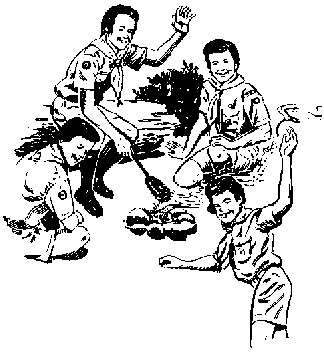
\includegraphics[width=3cm]{grafiki/happy.png}
  \end{center}
\end{wrapfigure} Podobnie jest i w  harcerstwie. Mimo, że wszystkim nam  chodzi o to samo, coś sprawia że harcerze z 15 PDH, różnią się od tych z 1 ŁDH. To  coś  to  nie  tylko  barwy i numer, ale wszystko to, co jest językiem i kulturą drużyny - obrzędy.
	Po co komu obrzędy? Jest  kilka  odpowiedzi:
\begin{itemize}[noitemsep,nolistsep] 
\item  tradycja --- ludzie się zmieniają,  świat się zmieni,  ale obyczaje zostaną;
\item  język --- którym mówi się chłopakom o co tu  właściwie chodzi;
\item  dyscyplina --- ułatwia techniczne prowadzenie np. zbiórki czy ogniska;
\item  jedność --- my mamy swoje obrzędy;
\item  przyciąganie ---  tajemnica intryguje;
\item  i wiele innych rzeczy.
\end{itemize}
	Czy tylko drużyna może posiadać obrzędowość? Nie, oczywiście także zastępy muszą mieć swoje obyczaje. Ale:
	\begin{itemize}[noitemsep,nolistsep] 
\item  muszą one współgrać z obyczajami drużyny
\item  nie może być  ich zbyt  dużo  aby  nie  przytłaczały
\item  muszą być nijako przy  okazji - chłopacy nie mogą całą zbiórkę wkuwać obrzędów
\item  nie wolno ich zmieniać bez powodu.
\end{itemize}
\begin{wrapfigure}{l}{4cm}
\begin{center}
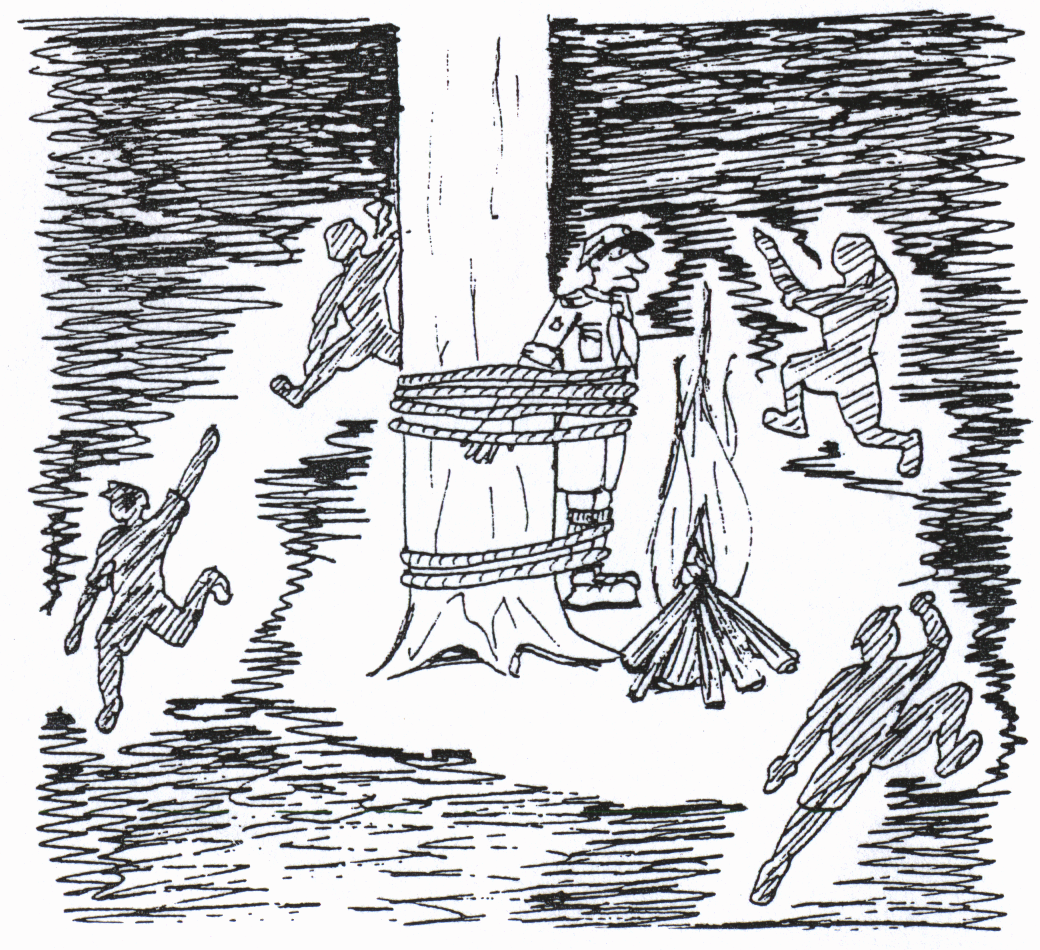
\includegraphics[width=4cm]{grafiki/drzewo.png}
\end{center}
\end{wrapfigure}Obrzędy i obyczaje  mogą  być  bardzo  różne:  od  sposobu  noszenia  proporca, przez  jakiś  znak  zastępu,  do  koloru  sznurowadeł  funkcyjnych zastępu  włącznie.  Ale uwaga! Obrzędowość nie  może być zbędnym balastem - musi pomagać, a nie  przeszkadzać.

Kiedy chcesz stworzyć nowy obrzęd,  zastanów się po co chcesz to  zrobić. 
 
\clearpage	
\section{Zbiórka zastępu}

Pytasz sam siebie: po co nam właściwie te zbiórki? 
Niezbyt kulturalnie można by odpowiedzieć pytaniem: a po co Wam właściwie harcerstwo?

Po to, żeby co dzień być trochę lepszym, trochę więcej umieć, trochę więcej wiedzieć, żeby  w końcu spędzić  sensownie czas, a to wszystko w kontekście celu wychowawczego ZHRu, o którym mówiliśmy już wcześniej.
	
No więc zostawił Cię Twój  okrutny drużynowy z zadaniem  przygotowania  zbiórki. 
Im bliżej terminu tym bardziej się denerwujesz. 
A może by tak nie pójść? 
Udać chorego? 
Eee\ldots

\begin{figure}[h]
\begin{center}
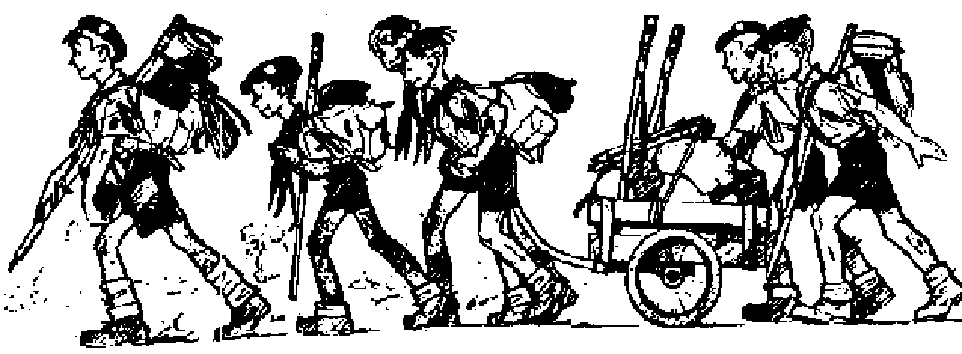
\includegraphics[width=0.9\textwidth]{grafiki/zbiorka.png}
\end{center}
\end{figure}
	
Siadasz w końcu nad kartką i rozmyślasz co by tu zrobić. Coś tam piszesz i  idziesz na zbiórkę. 
	
A może użyć  na  początek  takiego schematu:

Po co, czyli jaki \textbf{SENS} ma ta zbiórka? 
(kiedy chłopacy wrócą ze zbiórki muszą jednym zdaniem powiedzieć co robili: pełnili służbę w domu dziecka, grali w piłkę, zdobywali sprawności, odwiedzali super człowieka, harcowali po lesie) 
Pamiętaj, że oni zaraz wyczują, że zbiórka jest  tylko posklejana bez ładu z różnych gier.

Musi być \textbf{POMYSŁ}. czasem szalony, nierealny, ale porywający. Zrobić grę w niedostępnej części muzeum, odwiedzić drużynowych Twojej drużyny z ostatnich dziesięciu lat, zaprosić komandosa, urządzić bieg na podstawie aktualnego filmu z Jamesem Bondem, wleźć na czubek ratusza\ldots

Żeby to przeprowadzić musi być \textbf{PLAN}, czyli jak wprowadzić w życie mój (nasz) pomysł.
Gra  wg filmu Na  krawędzi z Sylwestrem Stallone:
\begin{enumerate}[noitemsep,nolistsep] 
\item spotkanie na Cytadeli;
\item szukanie walizki z milionem dolarów wg planu rozdanego wcześniej;
\item pokonanie przeciwników podczas podejścia pod najwyższą możliwą górę (a jak  się  ich  pokonuje?);
\item odnalezienie walizki z \ldots czekoladą w środku.
\end{enumerate}
A jaki był  sens tej zbiórki? 
O choćby ćwiczenia fizyczne podczas gonitwy, nauka czytania planu, podchodzenia, uczciwa walka itd.
	
Dużo czasu  zajmuje \textbf{PRZYGOTOWANIE} , ale nie zawsze sam musisz  rysować plan, przynosić walizkę i czekoladę, tasiemki do zrywania w pojedynkach. 
Rozdziel zadania.

Wróciłeś ze zbiórki. Podobało  się chłopakom?
Zapytaj siebie, czy gdybyś jej nie  przygotował, ale uczestniczył w takiej zbiórce przyszedłbyś na następną?
	
Może zapomniałeś o \textbf{ATMOSFERZE}? 
Ona nie zależy od terenu, miejsca. 
Ona zależy  od Ciebie! 
Traktowałeś wszystkich równo? 
Nie darłeś się na harcerzy? 
Opowiedziałeś kawał? 
To właśnie powoduje, że zbiórka nie jest lekcją!!!
\begin{wrapfigure}{l}{3cm}
\begin{center}
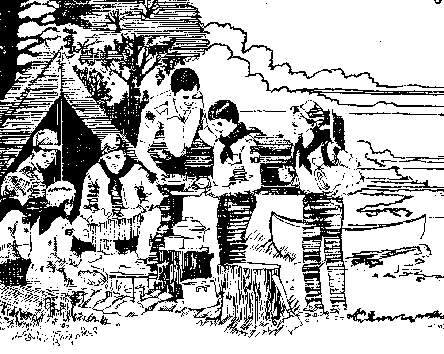
\includegraphics[width=3cm]{grafiki/zbiorkazastepu.png}
\end{center}
\end{wrapfigure}
\section{Zasady dobrej (Twojej) zbiórki}

Kiedy już opracujesz plan swojej zbiórki możesz sprawdzić czy zachowane są poniższe zasady. Nie przygotowuj zbiórki patrząc na tę ściągę. Czasem trzeba z któreś zasady zrezygnować na rzecz innej. Oceń swój plan i już  przeprowadzoną zbiórkę z tą listą. Wkrótce Twoje plany same się z nią zgodzą - nie będziesz już potrzebował ściąg.
\begin{description}


\item
[ZASADA 1 ZBIÓRKA MA LOGICZNY  CIĄG]
Jeden element zbiórki wypływa z drugiego. 
Z gawędy gra. 
Z gry - nauka  technik. 
Z technik - znów gra. 
Z gry - piosenka i tak dalej. 
Jeśli o tym zapomnisz, to ciągle będziesz zerkał do kartki z przygotowaną zbiórką (lekcje?),  a chłopcy zawsze to wyczują. 
Oni nie lubią drętwych zbiórek.
\item 
[ZASADA 2 CHARAKTER ZAJĘĆ MUSI  SIĘ ZMIENIAĆ]
Kiedy planujesz zbiórkę pamiętaj, że zbyt jednolite zajęcia nużą. 
Szybciej  spokojne, ale ruchowe także. 
Więc tak pozmieniaj kolejność zajęć  żeby mieszały się powaga (gawęda) z wesołością (piosenka), cisza (kominek) z hałasem (okrzyk  zastępu) spokój (praca rąk) z ruchem (gra ruchowa, turniej) dyscyplina (musztra, apel)  z luzem (zwiad,  gra).
\item
[ZASADA 3 ZBIÓRKA MUSI MIEĆ TEMPO]
Zanim ktokolwiek zapyta: czemu ta przerwa?, Ty musisz już przedstawić następny punkt programu. W czasie prowadzenia  gry,  mówienia gawędy i ćwiczenia węzłów, patrz czy  chłopcy się nie kręcą, nie zaczynają opowiadać kawałów. 
Wtedy  przerwij nawet jeśli nie zrobiłeś wszystkiego. 
Kończ  zbiórkę zanim się znudzą, wtedy chętniej przyjdą na następną.
\item
[ZASADA  4 ZASTĘPOWY JEST Z NAMI]
Nie siedź  z boku przyglądając się harcerzom. 
Weź udział w grze, najgłośniej się wydzieraj w okrzyku zastępu. 
Nie baw się w dyrektora, bądź jednym  z nich.
\item
[ZASADA  5 ZBIÓRKA  MA  CZTERY  STAŁE  ELEMENTY]
Obrzęd powitania, gawęda - to może być  wizyta fajnej osoby, dyskusja lub ciekawie opowiedziana historia - 5 minut to dosyć, nigdy nie przekraczaj 10 minut (5 minut gawędy to 20 minut jej przygotowywania w domu!), Rada Zastępu - tu  przekażesz sprawy bieżące,  tu  rozwiążecie wspólny problem, pomyśl nad obrzędem rozpoczęcia (może np. postawicie między Wami proporzec zastępu?), niech Rada trwa nie dłużej niż 15 minut, obrzęd pożegnania -  może jakiś specjalny Wasz krąg, krótka piosenka, może coś jeszcze innego?
\item
[ZASADA  6 COŚ NOWEGO I COŚ STAREGO NA KAŻDEJ ZBIÓRCE]
To chyba jasne? 
Przez przypomnienie znanych rzeczy, łączysz zbiórkę z poprzednią, wprowadzasz klimat. 
Możesz też utrwalić, przypomnieć to, co łatwo  się  zapomina.
\item
[ZASADA 7 NIE MA ZBIÓRKI BEZ INICJATYWY CHŁOPAKÓW]
Ciesz się kiedy chłopcy mają własne pomysły, chcą nagle przypomnieć starą grę, ulubioną piosenkę, zmienić przeprowadzaną przez Ciebie zabawę. 
To znaczy, że traktują zbiórkę jak swoją, chcą żeby była jak najfajniejsza. 
Nie możesz ich wiecznie pouczać, dyrygować  nimi. 
Jeśli w czasie zbiórki zdarzy się coś niezwykłego nie trzymaj się kurczowo napisanego  planu, ale wykorzystaj okazję żeby coś nowego poznać, zobaczyć, a zwłaszcza zrobić dobry  uczynek.
\item
[ZASADA  8 ZAWSZE DZIELIMY PRACĘ]
Jeśli zawsze sam przygotowujesz zbiórkę, to w końcu wyczerpią Ci się pomysły. Poza tym nauczysz harcerzy czekania na to, co będzie zamiast współtworzenia zbiórek.

Daj im zadania: przynieść tekst piosenki, życia do gry w terenie, busolę itd. Jeśli trzeba zaprosić gościa niech załatwią to chłopacy. Tylko pamiętaj: jeśli przed zbiórką nie zadzwonisz z pytaniem o wykonanie zadań, możesz się znaleźć w sytuacji, w której zabraknie Ci głównego punktu zbiórki!
\item
[ZASADA  9 NIESPODZIANKĘ ZAWSZE SIĘ WSPOMINA]
Staraj się przynajmniej co jakiś czas zaskoczyć mile chłopaków. Nie daj  im  pomyśleć,  że  wpadasz  w  rutynę i przyzwyczajenia.
	
	Co to może być? Musisz już sam wymyślić: ciekawą osobę, film video,  zbiórkę z zastępem harcerek...
\end{description}
	Że co? Że niby dużo tej teorii? Jeśli parę razy przygotujesz zbiórkę według  tych  paru zasad, same Ci  wejdą w krew i nawet nie będziesz wiedział kiedy i jak. Ale nie zaszkodzi  o jakiś czas tu zerknąć i  sobie  przypomnieć.
\begin{itemize}

\item ZASADA 1 - LOGICZNEGO  CIĄGU
\item ZASADA 2 - PRZEMIENNOŚCI ELEMENTÓW ZBIÓRKI
\item ZASADA 3 - TEMPA
\item ZASADA 4 - ZASTĘPOWY TEŻ JEST Z NAMI
\item ZASADA 5 -  CZTERECH  STAŁYCH  ELEMENTÓW ZBIÓRKI
\item ZASADA 6 -  COŚ  STAREGO I  COŚ NOWEGO NA ZBIÓRCE
\item ZASADA 7 -  SAMODZIELNOŚCI I INICJATYWY CHŁOPCÓW
\item ZASADA 8 - PODZIAŁU PRACY
\item ZASADA 9 - POZYTYWNEGO ZASKOCZENIA I NIESPODZIANKI

\end{itemize}
Na koniec coś co może Tobie  ułatwić planowanie zbiórek. To formy pracy:

Formy podstawowe:
-  ognisko	-  gawęda	- pląs 		- ćwiczenie
- okrzyk 	-  pokaz		- kominek	- zwiad
-  śpiewy	-  zadanie	- popis		- quiz
-  szkolenie	-  bieg		- turniej		- dyskusja
- rozmowa	-  obrzędy	- festiwal	- zawody
-  apel		-  musztra	- praca rąk	- próba
- gra		- harc		- alarm		-  podchody
- konkurs	- herbatka	- służba
- zadania zespołowe		- zadania międzyzbiórkowe
- działania społeczne			

Formy złożone :
-  zbiórka	-  obóz		-  biwak		-  włóczęga
-  zlot		-  kolonia	-  wycieczka	-  zimowisko
-  rajd		-  złaz


\section{Konflikty i problemy w zastępie}



\begin{wrapfigure}{l}{3cm}
\begin{center}
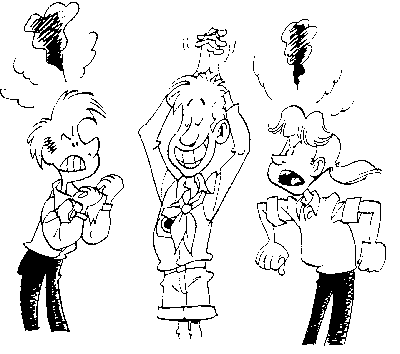
\includegraphics[width=3cm]{grafiki/konflikty.png}
\end{center}
\end{wrapfigure}\begin{aquote}{Ernst Bloch}
Rekin i słoń nie mogą się spotkać i nie stoczą ze sobą walki. Ale już wszystko, co żyje w tej samej wodzie, czy chce czy nie chce, tworzy jedność, w której możliwa jest i wojna i porozumienie
 \end{aquote}


Nie  wszystko  zawsze w  zastępie  funkcjonuje idealnie. 
Zresztą  dobrze  jest  gdy  w  zastępie  zdarzają się od czasu do  czasu burze,  byle tylko  dobrze  się kończyły.  Problemów, które  zwykle  jak  grom z  jasnego nieba spadają na zastępowego może być bardzo wiele. Jeden z chłopców często opuszcza  zbiórki, dwóch innych chce zmienić  zastęp,  a w ogóle to wszyscy o byle co  się kłócą itp.
	Jak z tym sobie radzić?  Sposobów jest bardzo wiele, często wybiera się ucieczkę, ignorowanie (niezauważanie problemu lub celowe jego pomijanie) jako metodę rozwiązania konfliktu, że nie są  to idealne  sposoby  zaradzania  problemom, nie trzeba chyba  specjalnie  przekonywać bo ucieczka czy ignorowanie zwykle kończy się rozbiciem zastępu lub bezsensowną rezygnacją zastępowego z pełnionej funkcji. Przecież Ty jesteś zastępowym bo umiesz sobie radzić z konfliktami  i  problemami lepiej niż inni. to garść dobrych rad, które powinny pomóc Wam rozwiązywać  konflikty, nie tylko te w zastępie ale także w  życiu.

1.
Trzeba zdać sobie sprawę, że problemy i konflikty zarówno w  życiu jak i w zastępie są nieuniknione.

2.
Problem trzeba zauważyć, a więc trzeba mieć oczy i uszy otwarte.

3.
Zadaj sobie pytanie: dlaczego? Jaka jest przyczyna problemu, konfliktu.

4.
Szukaj prawdziwej odpowiedzi na powyższe pytania, nie daj  się zwieść temu co mówią inni, lub czym Tobie oczy  mydlą  strony konfliktu. Czasem potrzeba Twardej konfrontacji poglądów z zainteresowanymi stronami konfliktu.
5.
Rozwiązanie konfliktu spróbuj znaleźć sam, gdy będziesz wiedział  gdzie naprawdę tkwi problem nie powinno to być trudne, jeśli nie możesz sobie poradzić sam, jest zawsze  gotowy Twój  starszy brat - drużynowy.

6.
Ostateczne rozwiązanie problemu dobrze jest przegadać z drużynowym. Czasem wręcz konieczna jest interwencja drużynowego  w  problem, szczególnie gdy do konfliktu dochodzi między Tobą – zastępowym, a którymś z  chłopaków.


Pamiętajcie, że wyrzucenie kogoś z zastępu z powodu jakiś niejasnych nieporozumień, czy konfliktów to jest nasza porażka. Spróbujmy teraz prześledzić wg  powyższego  wzoru jeden prosty konflikt. Jeden z harcerzy - niech będzie Jasio, nagle przestał przychodzić na zbiórki zastępu. Niby nic, ale w pewnym momencie drużynowy zaczyna zastępowemu wiercić dziurę w brzuchu w  sprawie Jasia.

1.
Warunek  pierwszy  został   spełniony,  mamy  problem.

2.
Być  może  zastępowy  sam zauważył problem ale na niego nie  zareagował, więc drużynowy pokazał go zastępowemu. 

3.
Teraz zastępowy sam musi się zastanowić:  dlaczego Jasio nie  przychodzi na zbiórki? Może dlatego,  że ma problemy w  szkole,  może  jest chory, może któryś z chłopaków bardzo mu na zbiórkach dokucza,  może... Każdy problem trzeba przeanalizować. Zastępowy myślał i nagle spojrzał do  swojego notatnika zastępowego i zobaczył, że jeszcze dwa miesiące  temu na  zbiórki przychodził cały zastęp - 8 osób,  a teraz  na  zbiórkach bywa 4 - 5 chłopców, czyli inni też  opuszczają  zbiórki,  może  tylko nie tak często jak nasz Jasio. Więc może zbiórki są mało  ciekawe,  chłopcy  się na nich dobrze nie czują...

4.
Swoją teorię powinien zastępowy sprawdzić  w rozmowie z chłopakami, a szczególnie z Jasiem. Okazało się, że miał  rację,  zbiórki  stały się mniej atrakcyjne, a ponadto Jasio ma problemy w szkole  z matmy.

5.
Zastępowy poznał problem,  teraz trzeba go tylko rozwiązać. Zbiórki powinny stać się bardziej  atrakcyjne. Odpowiedź na pytanie, jak to  robić,  znalazłeś w innej  części tego notatnika. Może warto każdą zbiórkę przygotowywać wspólnie z jednym z chłopaków,  za każdym razem  z innym? Co do problemów Jasia z matmą, przecież jego zastępowy ma 6 z matmy co za problem dać mu dwa razy  w tygodniu korki,  poprawi  oceny i  znów  może  przychodzić na  zbiórki.

6.
Rozwiązanie problemu gotowe, ale warto pogadać o tym z drużynowym. To drużynowy powinien porozmawiać  z rodzicami Jasia i zaproponować takie, czy inne rozwiązanie problemu.


\section{Nagrody i kary}
Między  karami i nagrodami musi być odpowiednia równowaga. Nie można tylko karać, tak jak samo nagradzanie nie rozwiąże wszystkich problemów. Pamiętajcie o tym, że fakt, iż musimy chłopaka z zastępu ukarać wynika często z naszego niedopatrzenia. Jeżeli chłopak robi coś źle, np. wycina swoje  inicjały w drzewie, to może nikt  mu nie  wytłumaczył, że  takie postępowanie nie przystoi harcerzowi.
\begin{wrapfigure}{l}{3cm}
\begin{center}
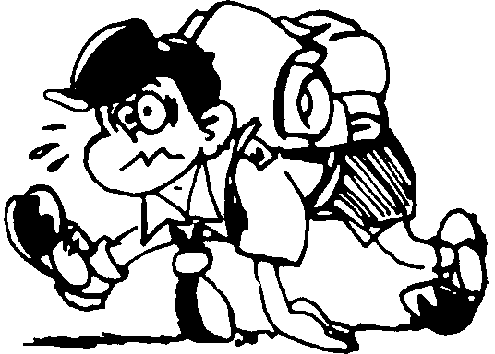
\includegraphics[width=3cm]{grafiki/plecak.png}
\end{center}
\end{wrapfigure}
Czasem, gdy chłopak coś przeskrobie wystarczy szczera męska rozmowa w cztery oczy. Gdy jednak to nie wystarcza może trzeba zwrócić uwagę chłopakowi przy pozostałych harcerzach zastępu  np. podczas wieczornego podsumowania dnia w zastępie. Czasem i ten sposób zawodzi albo przewinienie jest takie, że trzeba winnego  ukarać. Wówczas pamiętajcie, że każda kara musi mieć sens! Za każdym razem wytłumaczyć musicie dokładnie za  co  jest kara i na  czym  ma  ona polegać. Chciałbym Wam zaproponować dwa sposoby  karania.

Pierwszy to odsunięcie harcerza od pracy,  tzn. chodzi z zastępem wszędzie ale nie bierze udziału w tym co zastęp robi, a czas kary powinien wykorzystać na przemyślenie swojego błędu. 

Drugi sposób to dać możliwość naprawienia szkody którą wyrządził. Jeśli okaleczył drzewo, to niech pójdzie do leśniczego i jeden dzień przepracuje przy pielęgnacji szkółki leśnej, a wieczorem zda raport ze swojej pracy i przemyśleń nad złem które wyrządził. Jeśli zniszczył drugiemu prycz w namiocie niech ją podczas ciszy poobiedniej naprawi, a dodatkowo wykona jakiś element wyposażenia do namiotu zastępu. Niech kara którą wymierzacie uczy szacunku do pracy, przyrody i innych.

Pamiętajcie! Służba nie powinna być karą. Pełnić służbę to zaszczyt, choćby była trudna i niewdzięczna. Również nie mają większego sensu kary  w stylu biegania z plecakami, czy  robienia iluś tam pompek. Takie kary to ostateczność.

Nagrody. Nagradzaj każde dobre postępowanie harcerza. Niech by to była tylko ustna pochwała, ale przy  wszystkich członkach zastępu. Wytłumacz wówczas co takiego dobrego było w postępowaniu nagradzanego chłopaka. Dasz  innym wzór do naśladowania. Staraj się unikać nagród rzeczowych  w  stylu  np. ktoś przychodzi wzorowo umundurowany na zbiórkę to dostaje czekoladę. Doprowadzisz tylko do tego, że bez konkretnej nagrody chłopcy nic nie zrobią. Możesz np. chłopakowi, który przyszedł wzorowo umundurowany na zbiórkę pozwolić dokonać przeglądu mundurowego zastępu, w tym także Twojego  umundurowania.  a  pewno będzie  dumny, że mógł  sprawdzić   samego  zastępowego, a inni z pewnością będą mu nieco  zazdrościli.

Na koniec jedna ważna uwaga! Jeżeli chcecie ukarać lub nagrodzić kogoś zróbcie to jak najszybciej, a więc zaraz po zdarzeniu, wówczas chłopcy dokładnie wiedzą za co jest kara czy nagroda. Jeśli pochwalicie kogoś w czerwcu za to, że przyszedł na zbiórkę w lutym wzorowo umundurowany, to nikt nie będzie już  tego pamiętał, a z pewnością nikt nie będzie pamiętał jak był ten chłopak umundurowany, więc odpadnie możliwość naśladowania. Nagroda podobnie jak kara ma wychowywać, czyli mieć jakiś sens!

Zastanów się, jakbyś ukarał harcerza ze swojego zastępu, który ukradł na obozie  koledze czekoladę (i zjadł  ją sam), a jak ukarał byś harcerza, który podczas gry  oszukiwał i nie trzymał się wcześniej ustalonych zasad?

\begin{figure}[h]
\begin{center}
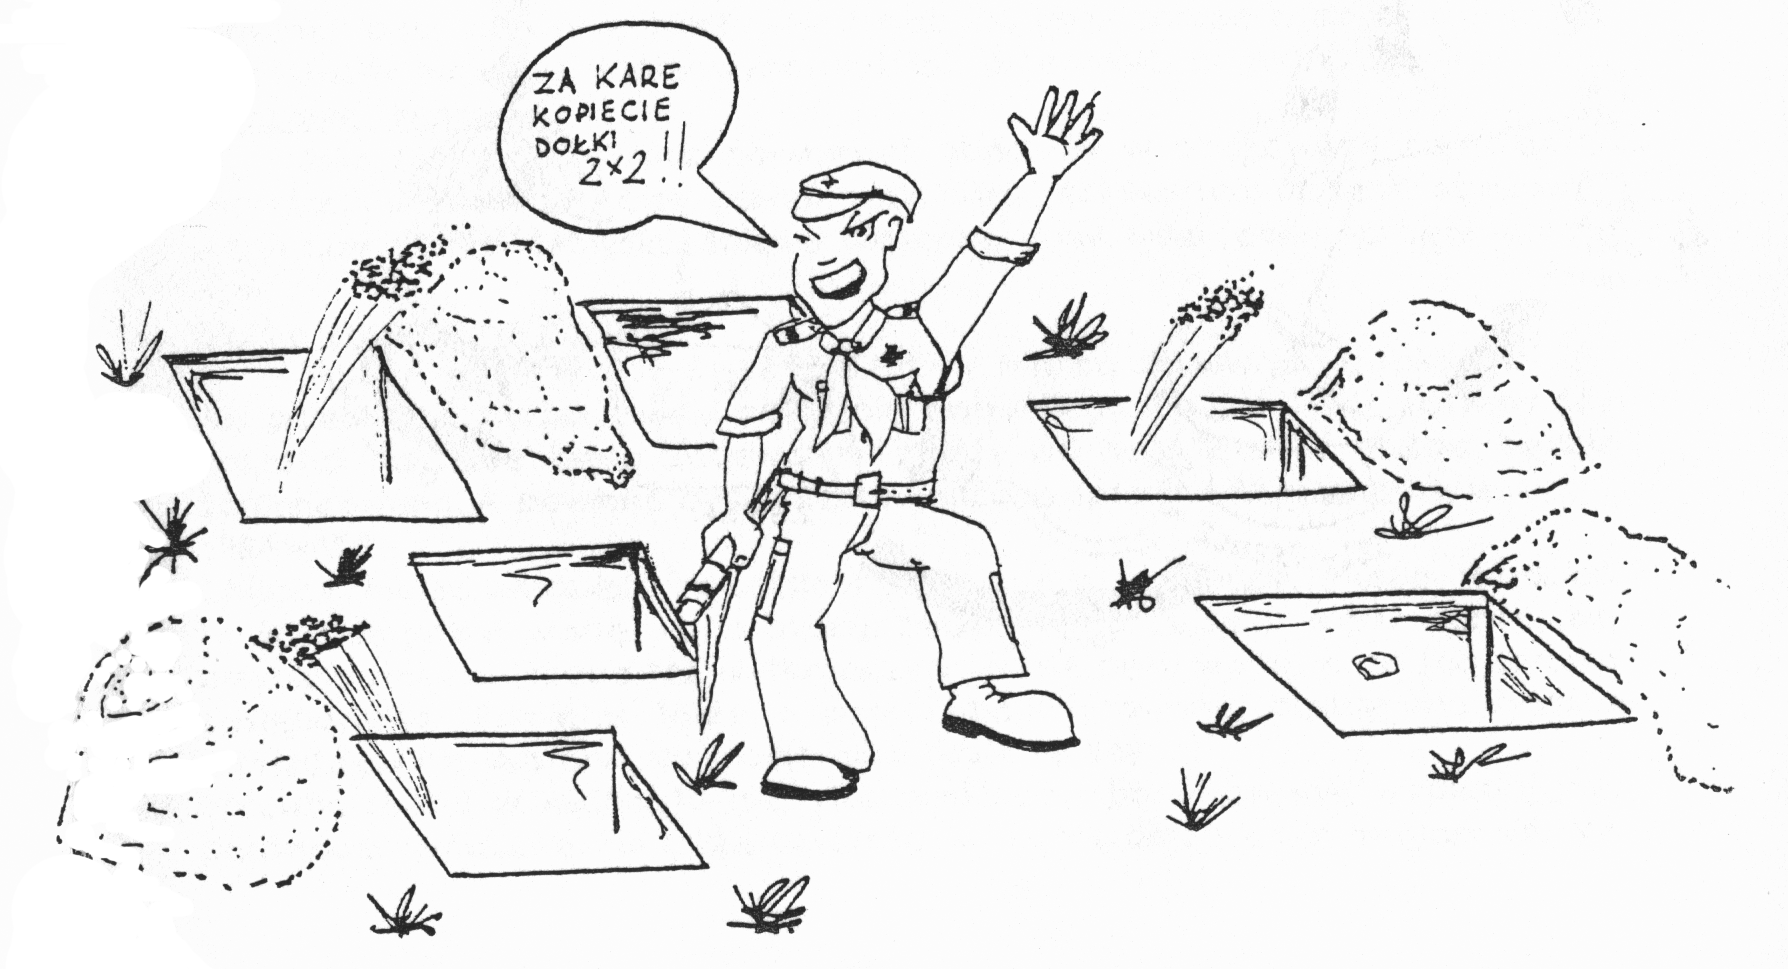
\includegraphics[width=0.9\textwidth]{grafiki/kara.png}
\end{center}
\end{figure}
	


\section{Sieć alarmowa zastępu}
\begin{wrapfigure}{l}{3cm}
\begin{center}
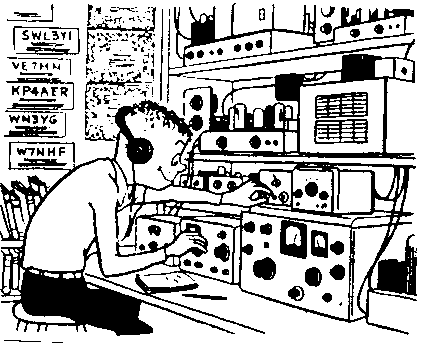
\includegraphics[width=3cm]{grafiki/nasluch.png}
\end{center}
\end{wrapfigure}Sieć alarmowa to sposób szybkiego przekazywania informacji pomiędzy kreślonymi osobami (członkami drużyny zastępu), przy użyciu najnowszych osiągnięć techniki (telefon, internet, łącza satelitarne, rower, samolot  itd.) oraz najstarszych darów natury (nogi, ręce, struny głosowe itd.). Bez łączności z tym, kto z nami wchodzi na szczyt, na pewno się tam nie dostaniemy. Sieć alarmową powinien posiadać każdy zastęp i drużyna, ponieważ bardzo ułatwia on pracę w drużynie oraz pozwala na zaoszczędzenie pieniędzy drużynowego lub zastępowego (na  telefony)  i czasu (potrzebnego na odwiedzenie i przekazanie informacji 150 harcerzom).

\begin{figure}[h]
\begin{center}
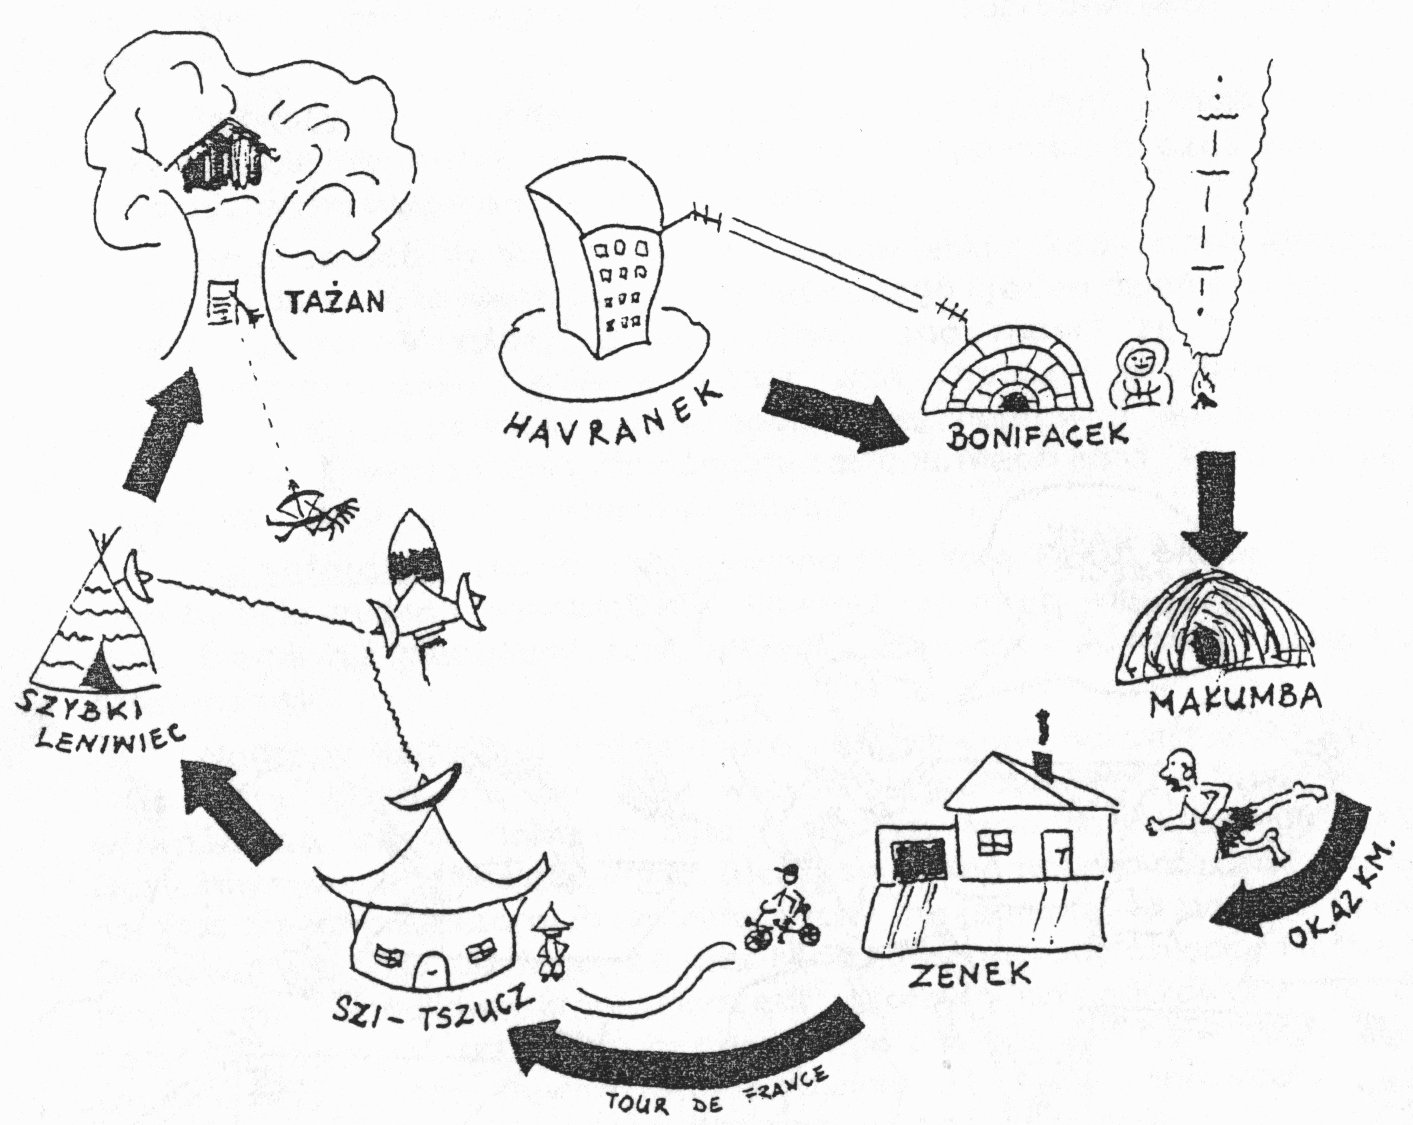
\includegraphics[width=0.9\textwidth]{grafiki/siec.png}
\end{center}
\end{figure}


\section{Zastęp na obozie}
To najlepszy okres w pracy zastępu. Dlaczego? Bo cały zastęp jest razem, przez  24 godziny na dobę, przez niemal cały miesiąc. Podczas dobrze przygotowanego obozu z zastępem możesz zrobić więcej, niż przez cały rok dobrej pracy.
	Warunkiem podstawowym jest, by zastępowy jechał na obóz! Bo to zastępowy przekazuje swoje umiejętności i wyrobienie pozostałym harcerzom zastępu:

- chłopacy mogą nie umieć rozbić namiotu, rozpalić ogniska, oprawić młotka. Ale zastępowy? Powinieneś im to  pokazać i pomóc.

- chłopcy mogą nie umieć odpowiednio (jak na harcerzy przystało) zachować się. Ale zastępowy ? Ty powinieneś być wzorem godnym naśladowania. Twoi harcerze z zastępu obserwują i naśladują Cię dzień i noc. Jeżeli Ty nawalisz oni także!

- chłopcy mogą się czasem obijać lub lenić. Ale zastępowy? Jako zastępowemu nie przystoi Tobie leżeć na kocu i wydawać  polecenia. Pracuj z całym zastępem, bardziej niż inni harcerze.

- chłopcy mogą nie wiedzieć jak najlepiej pełnić służby. Ale zastępowy? Ty organizujesz  służby rozdzielasz zadania, planujesz warty Dąż  wraz  z całym  zastępem do tego by Wasze służby były najlepsze, wzorowe. Zależy to przede  wszystkim  od  Ciebie.

\subsection{Atmosfera  na  obozie}
	Dbaj o dobrą atmosferę. Problemy i konflikty są nieuniknione, rozwiązuj  je  sprawiedliwie. Niech uśmiech nie znika z  twarzy Twoich harcerzy, ale przede wszystkim z Twojej. Może warto wieczorem zrobić całym zastępem rachunek  sumienia (podsumowanie dnia) i wymieniać co było dobrze, a co było nie tak. Każdy może się wtedy  wypowiedzieć, przeprosić, pogodzić ...

\subsection{Obozowe imprezy}
	Jako  zastępowy - wódz  powinieneś  dbać, by  w  obozowych  zajęciach  i  imprezach  uczestniczył  cały  zastęp. Jeśli więc jest festiwal piosenki obozowej niech cały zastęp wymyśla i śpiewa piosenkę, a nie tylko jeden harcerz, czy Ty sam.

\subsection{Służba zastępu na obozie}
	Służba - warta  jest  zaszczytem. Nie można stosować jej jako kary. Jak  przebiegnie  służba  zależy  od  Ciebie  i oboźnego. To czy Twój  zastęp i czy pozostali harcerze będą  zadowoleni zależy  od tego, jak  ta służba będzie zorganizowana. A powinna być przeprowadzona  sprawnie i sprawiedliwie.
	
\textbf{SPRAWNIE}: Chłopcy muszą wiedzieć dlaczego i jakie mają obowiązki. Muszą  wiedzieć kiedy i jak pełnią wartę, kogo budzą, że nie wolno zejść  z  warty zanim nie przyjdzie zmiana. Trzeba też wytłumaczyć, jak się pełni wartę, a to już sprawa zastępowego. Pamiętaj  także o posiłku dla  wartownika, będzie mu bardzo przykro, jeśli nie  dostanie go  wcale albo dostanie zimny!

Sprawna służba w  kuchni to nie tylko punktualne posiłki, pięknie wyglądające,  pachnące  i  smaczne. To także czystość  w  kuchni, porządek w magazynie. Nie ma nic gorszego jak leżące wokół kuchni papiery, brudne gary, porozrzucane wszędzie drewno, obierki na ziemi!!! Postaw się od czasu, do czasu w roli inspekcji sanitarnej i wraz zastępem zrób generalny porządek. W  porządku  łatwiej  wszystko  znaleźć a więc  lepiej  i szybciej się  pracuje.

\textbf{SPRAWIEDLIWIE}: Nie  można dzielić zadań i wart tak aby mali dostawali najgorszą  robotę i najgorsze warty. Nie można też tylko popuszczać małym i robić z nich mamisynków. Twoją rolą jest by podział wart i zadań w trakcie służby był sprawiedliwy.

	Pamiętaj Druhu Zastępowy! Obóz to  wspaniała zabawa,  niesamowite przygody, wielkie przeżycia, służba która wcale nie musi być kulą u nogi. Bardzo dużo jednak zależy od Ciebie, jak to zorganizujesz. Pomóż oboźnemu i komendantowi, a obóz naprawdę może być świetny!
	Ja chociaż byłem oboźnym i komendantem obozów najlepiej wspominam te, na których byłem zastępowym!
